\documentclass[9pt,xcolor=svgnames,aspectratio=169]{beamer}

\usepackage{packages}

\title{Introduction to Lattice Quantum Gravity}
\author[Name]{Timo Jakobs}
%\subtitle{Subtitle}
\institute[uni]{Bethe Center for Theoretical Physics \\ University of Bonn}
\date{\today}
%\titlegraphic{\vspace{-0.5cm}\hfill\includegraphics[scale=0.23]{logo.png}}


\begin{document}
{
\setbeamercolor{background canvas}{bg=NavyBlue!50!DarkOliveGreen, fg=white}
\setbeamercolor{normal text}{fg=white}
\maketitle
}%This is the colour of the first slide. bg= background and fg=foreground
\metroset{titleformat frame=smallcaps}
%
% \begin{frame}{Outline}
%  \setbeamertemplate{section in toc}[sections numbered]
%  \tableofcontents[hideallsubsections]
% \end{frame}

% \section{TODO}
%
% \begin{frame}{TODO}
%   \begin{itemize}
%     \item Ziele Grenzwerte der Monte Carlo
%     \item Phasendiagram am Anfang
%   \end{itemize}
% \end{frame}
%
% \begin{frame}{TODO - Questions}
%   \begin{itemize}
%     \item Check and Add Sources
%     \item Explain what a Simplex is
%   \end{itemize}
% \end{frame}
\section{What the heck is quantum gravity anyway?}


\begin{frame}{What the heck is quantum gravity anyway?}
 \begin{columns}[onlytextwidth,t]
  \uncover<1->{\begin{column}{0.48\textwidth}
    \begin{block}{Classical Gravity}
     \vspace{0pt}
     Einstein Field equations:
     \begin{align*}
      \uncoverubrace<2->{\frac{8 \pi G}{c^4}}{\kappa}\uncoverubrace<2->{T_{\mu\nu}}{\substack{\text{stuff within} \\  \text{space-time}}} & = \uncoverubrace<2->{R_{\mu\nu} - \frac{1}{2} R g_{\mu\nu} + \Lambda g_{\mu \nu}}{\text{geometry of space-time}}
      \uncover<3->{\intertext{Einstein Hilbert Action (for $T_{\mu\nu} = 0$):}
      S_{EH} [g] & = -\frac{1}{2 \kappa} \int \mathrm{d}^4 x \sqrt{-\mathrm{det} \, g} \, (R - 2\Lambda)}
     \end{align*}
    \end{block}
   \end{column}}
  \begin{column}{0.48\textwidth}
   \uncover<4->{\begin{block}{Quantum Gravity}
     \vspace{0pt}
     Path integral formulation:
     \begin{align*}
      Z_E & = \int \mathcal{D} g \, \exp \left( - S[g]\right)
     \end{align*}
    \end{block}}
   \uncover<5->{\textbf{Problems}
    \begin{itemize}
     \item non renormalizable coupling expansion
     \item might still be asymptotically safe \\ $\Rightarrow$ non-pertubative approaches
    \end{itemize}}
  \end{column}
 \end{columns}
\end{frame}


\section{Regge Action}


\begin{frame}{What the heck is quantum gravity anyway?}
 \begin{columns}[onlytextwidth,t]
  \uncover<1->{\begin{column}{0.48\textwidth}
    \begin{block}{Classical Gravity}
     \vspace{0pt}
     Einstein Field equations:
     \begin{align*}
      \uncoverubrace<2->{\frac{8 \pi G}{c^4}}{\kappa}\uncoverubrace<2->{T_{\mu\nu}}{\substack{\text{stuff within} \\  \text{space-time}}} & = \uncoverubrace<2->{R_{\mu\nu} - \frac{1}{2} R g_{\mu\nu} + \Lambda g_{\mu \nu}}{\text{geometry of space-time}}
      \uncover<3->{\intertext{Einstein Hilbert Action (for $T_{\mu\nu} = 0$):}
      S_{EH} [g] & = \frac{1}{2 \kappa} \int \mathrm{d}^4 x \sqrt{-\mathrm{det} \, g} \, (R - 2\Lambda)}
     \end{align*}
    \end{block}
   \end{column}}
  \begin{column}{0.48\textwidth}
   \uncover<4->{\begin{block}{Quantum Gravity}
     \vspace{0pt}
     Path integral formulation:
     \begin{align*}
      Z_E & = \int \mathcal{D} g \, \exp \left( - S[g]\right)
     \end{align*}
    \end{block}}
   \uncover<5->{\textbf{Problems}
    \begin{itemize}
     \item non renormalizable coupling expansion
     \item might still be asymptotically safe \\ $\Rightarrow$ non-pertubative approaches
    \end{itemize}}
  \end{column}
 \end{columns}
\end{frame}


\begin{frame}{Triangulations}
 \begin{columns}
  \begin{column}{0.38\textwidth}
   \begin{block}{Discretisation of $Z_E$}
    \vspace{0pt}
    \uncover<1->{Approximate space-time Manifold by triangulation}
    \uncover<2->{\begin{align*}
      \underbrace{\int \mathcal{D}g}_{\substack{\text{Integral over possible} \\ \text{metric tensors}}} \longrightarrow \underbrace{\sum_T \frac{1}{C_T}}_{\substack{\text{Sum over possible}\\ \text{triangulations}}}
     \end{align*}}
    \uncover<3->{Only equilateral triangles (simplices)}
    \uncover<4->{\begin{align*}
      S_E & = -\kappa_2(\kappa) N_2 + \kappa_4(\kappa, \Lambda) N_4
     \end{align*}
     where $N_k$ is the number of $k$-simplices in  $T$}
   \end{block}
  \end{column}
  \begin{column}{0.60\textwidth}
   \begin{figure}
    \centering
    \only<1-2>{\includegraphics[width=\textwidth]{pics/triangulation-fib.png}
     \caption{Triangulation of $S_2$ obtained by the Fibonacci Lattice\\ \tiny{rendered with the fresnel library (\url{https://github.com/glotzerlab/fresnel})}}}
    \only<3-4>{\includegraphics[width=\textwidth]{pics/triangulation-ico.png}
     \caption{Triangulation of $S_2$ obtained from Icosahedron\\ \tiny{rendered with the fresnel library (\url{https://github.com/glotzerlab/fresnel})}}}
   \end{figure}
  \end{column}
 \end{columns}
\end{frame}


\begin{frame}{Pachner Moves}
 %Local Update Moves for Metropolis-Monte-Carlo simulations:
 \begin{columns}[onlytextwidth,t]
  \begin{column}{0.37\textwidth}
   \uncover<1->{\begin{block}{Local Update Moves}
     \vspace{0pt}
     (Some Bullet Points to Explain the ergodic nature of the Pachner moves)
    \end{block}}
  \end{column}
  \begin{column}{0.34\textwidth}
   \begin{block}{2D}
    \vspace{0pt}
    \uncover<2->{\input{tikz/2DPachner-1}}\\
    \vspace{1.0em}
    \uncover<3->{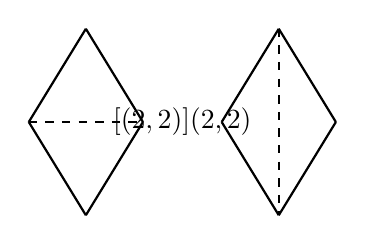
\begin{tikzpicture}
 \def\a{1.45}
 \def\b{0.5}
 \def\trigConst{0.816497}

 %1st Triangle
 \draw[thick, dashed] (-\a-\b,0) -- (-\b, 0);
 \draw[thick] (-\a-\b,0)         -- ({-\b-(0.5*\a)}, {\trigConst * \a});
 \draw[thick] (-\b,0)    -- ({-\b-(0.5*\a)}, {\trigConst * \a});
 \draw[thick] (-\a-\b,0)         -- ({-\b-(0.5*\a)}, {-\trigConst * \a});
 \draw[thick] (-\b,0)            -- ({-\b-(0.5*\a)}, {-\trigConst * \a});


 %2nd Triangle
 \draw[thick, dashed] ({\b+(0.5*\a)}, {\trigConst * \a}) -- ({\b+(0.5*\a)}, {-\trigConst * \a});
 \draw[thick] (\a+\b,0)                                  -- ({\b+(0.5*\a)}, {\trigConst * \a});
 \draw[thick] (\b,0)                                     -- ({\b+(0.5*\a)}, {\trigConst * \a});
 \draw[thick] (\a+\b,0)                                  -- ({\b+(0.5*\a)}, -{\trigConst * \a});
 \draw[thick] (\b,0)                                     -- ({\b+(0.5*\a)}, -{\trigConst * \a});

 %Lines to center

 \node[align=center] at (0,0) {$\xrightleftharpoons[(2,2)]{(2,2)}$};
\end{tikzpicture}
}
   \end{block}
  \end{column}
  \begin{column}{0.27\textwidth}
   \uncover<4->{\begin{block}{3D}
     \vspace{0pt}
     
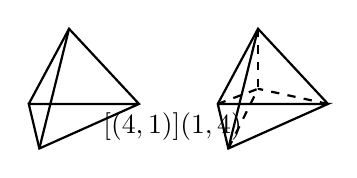
\begin{tikzpicture}[scale=1]
 \def\a{1.40}
 \def\b{0.5}
 \def\trigConst{0.816497}


 \begin{scope} [x     = {(1cm,0)},
   y     = {({0.7cm*cos(135)},{-0.7cm*sin(135)})},
   z     = {(0,1cm)}]

  \path coordinate (T1) at ({-(\b + (0.5*\a))}, {0.3333*\trigConst*\a}, {\trigConst*\a})
  coordinate (A1) at ({-\b},0,0)
  coordinate (B1) at ({-(\a + \b)},0,0)
  coordinate (C1) at ({-(\b + (0.5*\a))},{\trigConst*\a},0);


  \path coordinate (T2) at ({(\b + (0.5*\a))}, {0.3333*\trigConst*\a}, {\trigConst*\a})
  coordinate (A2) at ({\b},0,0)
  coordinate (B2) at ({(\a + \b)},0,0)
  coordinate (C2) at ({(\b + (0.5*\a))},{\trigConst*\a},0)
  coordinate (D2) at ({(\b + (0.5*\a))}, {0.3333*\trigConst*\a}, {0.3333*\trigConst*\a});


  \draw[thick]  (A1)  -- (B1) -- (C1) -- (A1) -- (T1) -- (B1);
  \draw[thick]  (C1) -- (T1);

  \draw[thick]  (A2)  -- (B2) -- (C2) -- (A2) -- (T2) -- (B2);
  \draw[thick]  (C2) -- (T2);

  \draw[thick, dashed] (A2) -- (D2);
  \draw[thick, dashed] (B2) -- (D2);
  \draw[thick, dashed] (C2) -- (D2);
  \draw[thick, dashed] (T2) -- (D2);

  \node[align=center] at ({0.15*\a},{0.5*\trigConst*\a},0) {$\xrightleftharpoons[(4,1)]{(1,4)}$};

 \end{scope}
\end{tikzpicture}
\\
     \vspace{1.0em}
     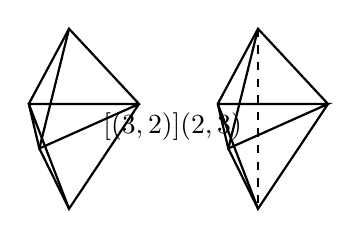
\begin{tikzpicture}[scale=1]
 \def\a{1.40}
 \def\b{0.5}
 \def\trigConst{0.816497}

 \begin{scope} [x     = {(1cm,0)},
   y     = {({0.7cm*cos(135)},{-0.7cm*sin(135)})},
   z     = {(0,1cm)}]


  \path coordinate (T1) at ({-(\b + (0.5*\a))}, {0.3333*\trigConst*\a}, {\trigConst*\a})
  coordinate (A1) at ({-\b},0,0)
  coordinate (B1) at ({-(\a + \b)},0,0)
  coordinate (C1) at ({-(\b + (0.5*\a))},{\trigConst*\a},0)
  coordinate (E1) at ({-(\b + (0.5*\a))}, {0.3333*\trigConst*\a}, {-\trigConst*\a});


  \path coordinate (T2) at ({(\b + (0.5*\a))}, {0.3333*\trigConst*\a}, {\trigConst*\a})
  coordinate (A2) at ({\b},0,0)
  coordinate (B2) at ({(\a + \b)},0,0)
  coordinate (C2) at ({(\b + (0.5*\a))},{\trigConst*\a},0)
  coordinate (D2) at ({(\b + (0.5*\a))}, {0.3333*\trigConst*\a}, {0.3333*\trigConst*\a})
  coordinate (E2) at ({(\b + (0.5*\a))}, {0.3333*\trigConst*\a}, {-\trigConst*\a});


  \draw[thick]  (A1)  -- (B1) -- (C1) -- (A1) -- (T1) -- (B1) -- (E1) -- (A1);
  \draw[thick]  (T1) -- (C1) -- (E1);

  \draw[thick]  (A2)  -- (B2) -- (C2) -- (A2) -- (T2) -- (B2) -- (E2) -- (A2);
  \draw[thick]  (T2) -- (C2) -- (E2);

  \draw[thick, dashed] (T2) -- (E2);


  \node[align=center] at ({0.15*\a},{0.5*\trigConst*\a},0) {$\xrightleftharpoons[(3,2)]{(2,3)}$};

 \end{scope}
\end{tikzpicture}

    \end{block}}
  \end{column}
 \end{columns}
 \center{\tiny{as e.g. found in INSERT SOURCE}}
 %https://arxiv.org/pdf/1412.8247.pdf
\end{frame}

\begin{frame}{Problems in four Dimensions}
 \begin{columns}[onlytextwidth,t]
  \begin{column}{0.48\textwidth}
   \begin{block}{Causal constraint (CDT)}
    \vspace{0pt}
   \end{block}
  \end{column}
  \begin{column}{0.48\textwidth}
   \begin{block}{Non trivial measure term}
    \vspace{0pt}
    Include non trivial measure term (SOURCE)
    \begin{align*}
     Z_E = \sum_T \frac{1}{C_T} \left[ \prod_{j=1}^{N_2} \mathcal{O} \left( t_j \right)^\beta \right] \mathrm{e}^{-S_E}
    \end{align*}
    with $\beta \neq 0$.
    \begin{itemize}
     \item $\mathcal{O}(t_j)$ is the \# 4-simplices the triangle $t_j$ belongs to
     \item Discrete limit of $\displaystyle \left[ \mathrm{det} (-g) \right]^{\beta/2}$
     \item Treat $\beta$ as another bare parameter
    \end{itemize}
   \end{block}
  \end{column}
 \end{columns}
\end{frame}


\section{Observables}


\begin{frame}{Phase Diagram of EDT}
 \begin{columns}
  \begin{column}{0.45\textwidth}
   \begin{align*}
    S_{ER} = - \kappa_2(\kappa,a) N_2 + \kappa_4(\kappa,\Lambda, a) N_4 + \lambda\abs{N_4 - V}
   \end{align*}
   \begin{block}{Physical Limits}
    \vspace{0pt}
    \begin{itemize}
     \uncover<2->{\item $\kappa_4$ sets scale and cosmological constant (continuum limit)}
           \uncover<3->{\item $V \rightarrow \infty$ for infinite Volume}
           \uncover<4->{\item $(\beta,\kappa_2) \rightarrow \infty$ just to the left of first order phase transition $\overline{AB}$}
    \end{itemize}
   \end{block}
  \end{column}
  \begin{column}{0.53\textwidth}
   \uncover<4->{\begin{figure}
     \includegraphics[width=\textwidth]{pics/phase-diagram}
     \caption{\tiny{As found in: Laiho, Bassler, Coumbe, Du, Neelakanta \emph{PhysRevD.96.064015}}}
    \end{figure}}
  \end{column}
 \end{columns}
\end{frame}

\begin{frame}{Vertex Count}
 \begin{figure}
  \centering
  \includegraphics[width=0.8\textwidth]{pics/VertexCount}
  \caption{\tiny{As found in: Laiho, Bassler, Coumbe, Du, Neelakanta \emph{PhysRevD.96.064015}}}
 \end{figure}
\end{frame}


\begin{frame}{Fractal Dimensions}
 \begin{columns}%[onlytextwidth,t]
  \begin{column}{0.35\textwidth}
   \begin{block}{Box Counting Dimensions}
    \vspace{0pt}
    \begin{align*}
     d_{\textrm{box}} & = \lim_{\epsilon \rightarrow 0} \frac{\log(N(\varepsilon))}{\log(1/\varepsilon)}
    \end{align*}\\
    (Similar to Hausdorf dimension $d_H$)
   \end{block}
  \end{column}
  \uncover<2->{\begin{column}{0.32\textwidth}
    \begin{block}{Line}
     \vspace{0pt}
     \begin{center}
      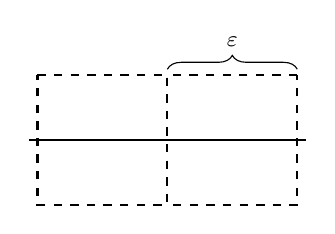
\begin{tikzpicture}
 \def\a{1.1}

 %Line
 \draw[thick] (-1.6*\a, 0) -- (1.6*\a, 0);

 %Boxes
 \uncover<3->{
  \draw[thick,dashed] (-1.5*\a, 0.75*\a) -- (0, 0.75*\a) -- (0, -0.75*\a) -- (-1.5*\a, -0.75*\a) -- (-1.5*\a, 0.75*\a);
  \draw[thick,dashed] (1.5*\a, 0.75*\a) -- (0*\a, 0.75*\a) -- (0*\a, -0.75*\a) -- (1.5*\a, -0.75*\a) -- (1.5*\a, 0.75*\a);
  \draw [decorate,decoration={brace,amplitude=5pt},yshift=2pt] (0, 0.75*\a) -- (1.5*\a, 0.75*\a) node [black,midway,yshift=0.35cm]
{\footnotesize $\varepsilon$};
 }

\end{tikzpicture}
\\
      \vspace{0.2cm}
      \uncover<4->{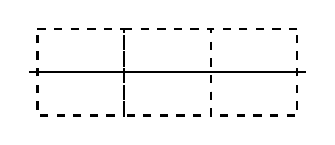
\begin{tikzpicture}
 \def\a{1.1}

 %Line
 \draw[thick] (-1.6*\a, 0) -- (1.6*\a, 0);

 %Boxes
 \draw[thick,dashed] (-1.5*\a, 0.5*\a) -- (-0.5*\a, 0.5*\a) -- (-0.5*\a, -0.5*\a) -- (-1.5*\a, -0.5*\a) -- (-1.5*\a, 0.5*\a);
 \draw[thick,dashed] (-0.5*\a, 0.5*\a) -- (0.5*\a, 0.5*\a) -- (0.5*\a, -0.5*\a) -- (-0.5*\a, -0.5*\a) -- (-0.5*\a, 0.5*\a);
 \draw[thick,dashed] (1.5*\a, 0.5*\a) -- (0.5*\a, 0.5*\a) -- (0.5*\a, -0.5*\a) -- (1.5*\a, -0.5*\a) -- (1.5*\a, 0.5*\a);

\end{tikzpicture}
}\\
      \vspace{0.2cm}
      \uncover<5->{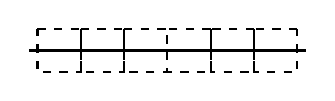
\begin{tikzpicture}
 \def\a{1.1}

 %Line
 \draw[thick] (-1.6*\a, 0) -- (1.6*\a, 0);

 %Boxes
 \draw[thick,dashed] (-1.5*\a, 0.25*\a) -- (-1.0*\a, 0.25*\a) -- (-1.0*\a, -0.25*\a) -- (-1.5*\a, -0.25*\a) -- (-1.5*\a, 0.25*\a);
 \draw[thick,dashed] (-1.0*\a, 0.25*\a) -- (-0.5*\a, 0.25*\a) -- (-0.5*\a, -0.25*\a) -- (-1.0*\a, -0.25*\a) -- (-1.0*\a, 0.25*\a);
 \draw[thick,dashed] (-0.5*\a, 0.25*\a) -- (0, 0.25*\a) -- (0, -0.25*\a) -- (-0.5*\a, -0.25*\a) -- (-0.5*\a, 0.25*\a);
 \draw[thick,dashed] (1.5*\a, 0.25*\a) -- (1.0*\a, 0.25*\a) -- (1.0*\a, -0.25*\a) -- (1.5*\a, -0.25*\a) -- (1.5*\a, 0.25*\a);
 \draw[thick,dashed] (1.0*\a, 0.25*\a) -- (0.5*\a, 0.25*\a) -- (0.5*\a, -0.25*\a) -- (1.0*\a, -0.25*\a) -- (1.0*\a, 0.25*\a);
 \draw[thick,dashed] (0.5*\a, 0.25*\a) -- (0, 0.25*\a) -- (0, -0.25*\a) -- (0.5*\a, -0.25*\a) -- (0.5*\a, 0.25*\a);


\end{tikzpicture}
}
     \end{center}
     \uncover<6->{\begin{align*}
       N(\epsilon) \sim \frac{1}{\varepsilon} \, \Rightarrow \, d_{\textrm{box}} & = 1
      \end{align*}}
    \end{block}
   \end{column}}
  \uncover<7->{\begin{column}{0.32\textwidth}
    \begin{block}{Plane}
     \vspace{0pt}
     \begin{center}
      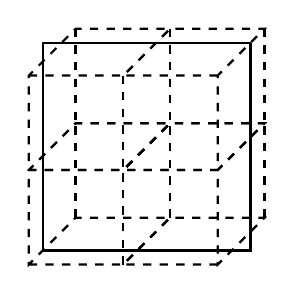
\begin{tikzpicture}[scale=1]
 \def\a{1.2}

 \begin{scope} [x     = {(1cm,0)},
   y     = {({0.7cm*cos(135)},{-0.7cm*sin(135)})},
   z     = {(0,1cm)}]

   \draw[thick] (1.1*\a,0.5*\a,1.1*\a) -- (-1.1*\a,0.5*\a,1.1*\a) -- (-1.1*\a,0.5*\a,-1.1*\a) -- (1.1*\a,0.5*\a,-1.1*\a) -- (1.1*\a,0.5*\a,1.1*\a);

  \draw[thick,dashed] (\a,\a,\a) -- (0,\a,\a) -- (0,0,\a) -- (\a,0,\a) -- (\a,\a,\a) -- (\a,\a,0) -- (0,\a,0) -- (0,0,0) -- (\a,0,0) -- (\a,\a,0);
  \draw[thick,dashed] (0,\a,\a) -- (0,\a,0);
  \draw[thick,dashed] (0,0,\a) -- (0,0,0);
  \draw[thick,dashed] (\a,0,\a) -- (\a,0,0);

  \draw[thick,dashed] (-\a,\a,\a) -- (0,\a,\a) -- (0,0,\a) -- (-\a,0,\a) -- (-\a,\a,\a) -- (-\a,\a,0) -- (0,\a,0) -- (0,0,0) -- (-\a,0,0) -- (-\a,\a,0);
  \draw[thick,dashed] (0,\a,\a) -- (0,\a,0);
  \draw[thick,dashed] (0,0,\a) -- (0,0,0);
  \draw[thick,dashed] (-\a,0,\a) -- (-\a,0,0);

  \draw[thick,dashed] (\a,\a,-\a) -- (0,\a,-\a) -- (0,0,-\a) -- (\a,0,-\a) -- (\a,\a,-\a) -- (\a,\a,0) -- (0,\a,0) -- (0,0,0) -- (\a,0,0) -- (\a,\a,0);
  \draw[thick,dashed] (0,\a,-\a) -- (0,\a,0);
  \draw[thick,dashed] (0,0,-\a) -- (0,0,0);
  \draw[thick,dashed] (\a,0,-\a) -- (\a,0,0);

  \draw[thick,dashed] (-\a,\a,-\a) -- (0,\a,-\a) -- (0,0,-\a) -- (-\a,0,-\a) -- (-\a,\a,-\a) -- (-\a,\a,0) -- (0,\a,0) -- (0,0,0) -- (-\a,0,0) -- (-\a,\a,0);
  \draw[thick,dashed] (0,\a,-\a) -- (0,\a,0);
  \draw[thick,dashed] (0,0,-\a) -- (0,0,0);
  \draw[thick,dashed] (-\a,0,-\a) -- (-\a,0,0);


 \end{scope}
\end{tikzpicture}
\\
     \end{center}
     \begin{align*}
      N(\epsilon) \sim \frac{1}{\varepsilon^2} \, \Rightarrow \, d_{\textrm{box}} & = 2
     \end{align*}
    \end{block}
   \end{column}}
 \end{columns}
\end{frame}

\begin{frame}{Box counting dimension}
 \begin{columns}[onlytextwidth,t]
  \begin{column}{0.48\textwidth}
   \begin{block}{Koch Snow Flake}
    \vspace{0pt}
    \begin{center}
     \begin{tikzpicture}[decoration=Koch snowflake]
 \def\a{0.2}

 %Fractals
 \uncover<1>{\draw[thick] (0,0) -- (27*\a,0);}
 \uncover<2>{\draw[thick] decorate{ (0,0) -- (27*\a,0)};}
 \uncover<3>{\draw[thick] decorate { decorate{ (0,0) -- (27*\a,0)}};}
 \uncover<4>{\draw[thick] decorate {decorate { decorate{ (0,0) -- (27*\a,0)}}};}
 \uncover<5->{\draw[thick] decorate {decorate {decorate { decorate{ (0,0) -- (27*\a,0)}}}};}

 %Coverings
 \only<6>{\draw[thick,dashed] (0,13.5*\a) -- (27*\a,13.5*\a) -- (27*\a,-13.5*\a) -- (0,-13.5*\a) -- (0,13.5*\a); }
 \only<7>{
  \draw[thick,dashed] (0, -4.5 * \a) -- (9*\a, -4.5 * \a) -- (9*\a, 4.5 * \a) -- (0, 4.5 * \a) -- (0, -4.5 * \a);
  \draw[thick,dashed] (9 * \a, -4.5 * \a) -- (18*\a, -4.5 * \a) -- (18*\a, 4.5 * \a) -- (9 * \a, 4.5 * \a) -- (9 * \a, -4.5 * \a);
  \draw[thick,dashed] (18 * \a, -4.5 * \a) -- (27*\a, -4.5 * \a) -- (27*\a, 4.5 * \a) -- (18 * \a, 4.5 * \a) -- (18 * \a, -4.5 * \a);
 }
 \uncover<7>{\draw[thick,dashed] (9 * \a, 4.5 * \a) -- (18*\a, 4.5 * \a) -- (18*\a, 13.5 * \a) -- (9 * \a, 13.5 * \a) -- (9 * \a, 4.5 * \a);}
 \only<8->{
  \draw[thick,dashed] (0, -1.5 * \a) -- (3*\a, -1.5 * \a) -- (3*\a, 1.5 * \a) -- (0, 1.5 * \a) -- (0, -1.5 * \a);
  \draw[thick,dashed] (3*\a, -1.5 * \a) -- (6*\a, -1.5 * \a) -- (6*\a, 1.5 * \a) -- (3*\a, 1.5 * \a) -- (3*\a, -1.5 * \a);
  \draw[thick,dashed] (6*\a, -1.5 * \a) -- (9*\a, -1.5 * \a) -- (9*\a, 1.5 * \a) -- (6*\a, 1.5 * \a) -- (6*\a, -1.5 * \a);
  \draw[thick,dashed] (6*\a, -1.5 * \a) -- (9*\a, -1.5 * \a) -- (9*\a, 1.5 * \a) -- (6*\a, 1.5 * \a) -- (6*\a, -1.5 * \a);
  \draw[thick,dashed] (9*\a, -1.5 * \a) -- (12*\a, -1.5 * \a) -- (12*\a, 1.5 * \a) -- (9*\a, 1.5 * \a) -- (9*\a, -1.5 * \a);

  \draw[thick,dashed] (3*\a, 1.5 * \a) -- (6*\a, 1.5 * \a) -- (6*\a, 4.5 * \a) -- (3*\a, 4.5 * \a) -- (3*\a, 1.5 * \a);
  \draw[thick,dashed] (9*\a, 1.5 * \a) -- (12*\a, 1.5 * \a) -- (12*\a, 4.5 * \a) -- (9*\a, 4.5 * \a) -- (9*\a, 1.5 * \a);

  \draw[thick,dashed] (9*\a, 4.5 * \a) -- (12*\a, 4.5 * \a) -- (12*\a, 7.5 * \a) -- (9*\a, 7.5 * \a) -- (9*\a, 4.5 * \a);


  \draw[thick,dashed] (15*\a, -1.5 * \a) -- (18*\a, -1.5 * \a) -- (18*\a, 1.5 * \a) -- (15*\a, 1.5 * \a) -- (15*\a, -1.5 * \a);
  \draw[thick,dashed] (18*\a, -1.5 * \a) -- (21*\a, -1.5 * \a) -- (21*\a, 1.5 * \a) -- (18*\a, 1.5 * \a) -- (18*\a, -1.5 * \a);
  \draw[thick,dashed] (21*\a, -1.5 * \a) -- (24*\a, -1.5 * \a) -- (24*\a, 1.5 * \a) -- (21*\a, 1.5 * \a) -- (21*\a, -1.5 * \a);
  \draw[thick,dashed] (24*\a, -1.5 * \a) -- (27*\a, -1.5 * \a) -- (27*\a, 1.5 * \a) -- (24*\a, 1.5 * \a) -- (24*\a, -1.5 * \a);

  \draw[thick,dashed] (15*\a, 1.5 * \a) -- (18*\a, 1.5 * \a) -- (18*\a, 4.5 * \a) -- (15*\a, 4.5 * \a) -- (15*\a, 1.5 * \a);
  \draw[thick,dashed] (21*\a, 1.5 * \a) -- (24*\a, 1.5 * \a) -- (24*\a, 4.5 * \a) -- (21*\a, 4.5 * \a) -- (21*\a, 1.5 * \a);

  \draw[thick,dashed] (15*\a, 4.5 * \a) -- (18*\a, 4.5 * \a) -- (18*\a, 7.5 * \a) -- (15*\a, 7.5 * \a) -- (15*\a, 4.5 * \a);


  \draw[thick,dashed] (12*\a, 4.5 * \a) -- (15*\a, 4.5 * \a) -- (15*\a, 7.5 * \a) -- (12*\a, 7.5 * \a) -- (12*\a, 4.5 * \a);
  \draw[thick,dashed] (12*\a, 7.5 * \a) -- (15*\a, 7.5 * \a) -- (15*\a, 10.5 * \a) -- (12*\a, 10.5 * \a) -- (12*\a, 7.5 * \a);

 }

\end{tikzpicture}
\\
    \end{center}
    \uncover<9->{\begin{align*}
      N(\epsilon) \sim \varepsilon^{-\log_3 (4)} & = \left(\frac{1}{\varepsilon}\right)^{ \frac{\log4}{\log3}} \\
      \Rightarrow \, \, d_{\textrm{box}}         & = \frac{\log 4}{\log 3} \approx 1.262
     \end{align*}}
   \end{block}
  \end{column}
  \begin{column}{0.48\textwidth}
   \uncover<10->{\begin{block}{Coastlines}
    \vspace{0pt}
    \begin{figure}
     \centering
     \includegraphics[width=\textwidth]{pics/Great_Britain_Box}
     \caption{\tiny{Source: \url{https://commons.wikimedia.org/wiki/File:Great_Britain_Box.svg}} }
    \end{figure}
    \uncover<11->{\vspace{-0.8cm}
     \begin{align*}
      d_{\textrm{box}} \approx 1.215
     \end{align*}}}
    %    % Germany: 1.111
    %    % United Kingdom: 1.215
    %    % Norway: 1.372
   \end{block}
  \end{column}
 \end{columns}
\end{frame}

\begin{frame}{Fractal Dimension of the triangulation}
 \begin{columns}
  \begin{column}{0.58\textwidth}
   \begin{block}{Scaling of different Observables as function of $N_4$}
    \vspace{0pt}
    \begin{align*}
     N_4^{\textrm{shell}} (\tau) = \parbox{0.55\textwidth}{\# four-simplices within spherical shell of radius $\tau$}
    \end{align*}
    \vspace{-0.4cm}
    \begin{itemize}
     %\item 3D volume as a function of euclidian time $\tau$
     \uncover<2->{\item Expect 3D volume to scale with $\sim (N_4)^{3/4}$}
           \uncover<3->{\item Expect Radius (1D volume) to scale with $\sim (N_4)^{1/4}$\\
           $\rightarrow$ scale invariant radius $\rho = 1/N_4^{1/d}$}
    \end{itemize}
    \uncover<4->{\begin{align*}
      N_4^{\textrm{shell}} \rightarrow n_4^{\textrm{shell}}(N_4,d) & = \frac{1}{N_4^{1-1/d}} N_4^{\textrm{shell}} (N_4^{1/d} \rho)
     \end{align*}
     Expect $n_4(N_4) = \mathrm{const}$ for $d=d_H$}
   \end{block}
  \end{column}
  \begin{column}{0.4\textwidth}
   \uncover<5->{\centering
   \begin{figure}
    \includegraphics[width=0.9\textwidth]{pics/Hausdorf1}
    %\includegraphics[height=0.47\textwidth]{pics/Hausdorf2}
    \caption{\tiny{As found in: Laiho, Bassler, Coumbe, Du, Neelakanta \emph{PhysRevD.96.064015}}}
   \end{figure}
   $\longrightarrow \quad d_H = 4.1 \pm 0.3$}
  \end{column}
 \end{columns}
\end{frame}

\begin{frame}{Classical Limit}
 \begin{columns}
  \begin{column}{0.48\textwidth}
   \begin{block}{de Sitter Solution}
    \vspace{0pt}
    \begin{itemize}
     \item symmetric vacuum solution of gravity
     \item equivalent to $S_3$ (in euclidian space-time)
           \begin{align*}
            \rightarrow n_4^{\textrm{shell}} (\rho) \sim \sin^3 \left(  \frac{\rho}{s_0(N_4)^{1/4}} \right)
           \end{align*}
    \end{itemize}
   \end{block}
   \uncover<3->{\begin{block}{Spectral Dimension}
    \vspace{0pt}
    \begin{itemize}
     \item Dimension defined by diffusion process
           \begin{align*}
            D_S = - 2 \frac{\mathrm{d} \log \left\langle P(\sigma) \right\rangle}{\mathrm{d} \log \sigma}
           \end{align*}
           with return $P(\sigma)$ probability after $\sigma$ diffusion steps
     \item $d_S \approx 4$ at large scales, $D_S \approx \frac{3}{2}$
    \end{itemize}
   \end{block}}
  \end{column}
  \begin{column}{0.48\textwidth}
   \uncover<2->{\begin{figure}
    \centering
    \includegraphics[width=0.8\textwidth]{pics/deSitter}
    \caption{\tiny{As found in: Laiho, Bassler, Coumbe, Du, Neelakanta \emph{PhysRevD.96.064015}}}
   \end{figure}}
  \end{column}
 \end{columns}
\end{frame}

\begin{frame}{Phase Diagram of EDT}
 \begin{columns}
  \begin{column}{0.48\textwidth}
   \begin{itemize}
    \uncover<2->{\item Collapsed Phase
          \begin{itemize}
           \item $d_H \rightarrow \infty$, $d_s \rightarrow \infty$
           \item Few strongly connected vertices
          \end{itemize}}
          \uncover<3->{\item Branched Polymer Phase
          \begin{itemize}
           \item $d_H = 2$, $d_S=\frac{4}{3}$
           \item Baby universe branching
          \end{itemize}}
          \uncover<4->{\item Crinkled region in between
          \begin{itemize}
           \item shares features of both previous phases
           \item no distinct phase transition
          \end{itemize}}
   \end{itemize}
   \vspace{0.2cm}
   \uncover<4->{Physical limit when following $\overline{AB}$ to $\infty$}
  \end{column}
  \begin{column}{0.48\textwidth}
   \uncover<1->{\begin{figure}
     \includegraphics[width=\textwidth]{pics/phase-diagram}
     \caption{\tiny{As found in: Laiho, Bassler, Coumbe, Du, Neelakanta \emph{PhysRevD.96.064015}}}
    \end{figure}}
  \end{column}
 \end{columns}
\end{frame}


\section{Conclusion}


\begin{frame}{Conclusion}
 \begin{columns}
  \begin{column}{0.57\textwidth}
   \begin{block}{Outlook}
    \vspace{0pt}
    \begin{itemize}
     \item Coupling to scalar fields shows Newtonian Binding\\
     {\tiny{Dai, Laiho, Schiffer, Unmuth-Yockey \emph{PhysRevD.103.114511}}}
     \item Extraction of the gravitational constant consistent between pure gravity and scalar fields\\
     {\tiny{Bassler, Laiho, Schiffer, Unmuth-Yockey \emph{PhysRevD.103.114504}}}
     % \item  Kähler Dirac Fermions on EDT\\
     % (Insert Paper Reference)
    \end{itemize}
    %$\rightarrow$ Quantum gravity seems to be asymptotically safe
    %$\rightarrow$ EDT seems to be a promising candidate for quantum gravity
   \end{block}
  \end{column}
  \begin{column}{0.42\textwidth}
   \begin{block}{Sources}
    \begin{itemize}
      \item Laiho, Bassler, Coumbe, Du, Neelakanta \emph{PhysRevD.96.064015}\\
            \emph{Lattice quantum gravity and asymptotic safety}
      \item Cuzinatto, de Melo, Naldoni de Souza \url{arxiv.org/abs/1904.01966}
            \emph{Introduction to Regge Calculus for Gravitation}
    \end{itemize}
   \end{block}
  \end{column}
 \end{columns}
\end{frame}


\begin{frame}
 \resizebox{0.5\textwidth}{!}{The End - Thanks for listening}\\
 \vspace{0.5cm}
 Code can be found at:
\end{frame}

\appendix

\input{sec_bonus}

\end{document}
